\documentclass{standalone}

\usepackage{tikz}
\usepackage{amssymb}
\usetikzlibrary{calc, positioning}
\begin{document}
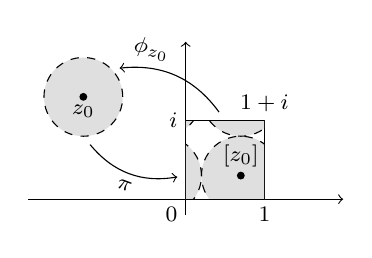
\begin{tikzpicture}[every node/.style={node font=\footnotesize}]
  \draw[->] (-2,0) to (2,0);
  \draw[->] (0,-0.2) to (0,2);

  \coordinate (z0) at (-1.3,1.3);
  \filldraw[dashed, fill=gray!50, fill opacity=0.5] (z0) circle (0.5);
  \fill (z0) circle (0.05) node[below]{$ z_0 $};
  \node (l) at ($ (z0) + (-90:0.5) $){};
  \node (l') at ($ (z0) + (45:0.5) $){};

  \begin{scope}
    \draw (0,0) rectangle (1,1);
      \node[below left] at (0,0){$ 0 $};
      \node[left] at (0,1){$ i $};
      \node[below] at (1,0){$ 1 $};
      \node[above] at (1,1){$ 1+i $};

      \node (r) at (0,0.3){};
      \node (r') at (0.5,1){};
    
    \clip (0,0) rectangle (1,1);

    \foreach \x in {-2,-1,...,2}{
      \foreach \y in {-2,-1,...,2}{
        \filldraw[dashed, fill=gray!50, fill opacity=0.5] ($(z0) + (\x,\y) $)
          circle (0.5);
        \fill ($(z0) + (\x,\y) $) circle (0.05) node[above]{$ [z_0] $};
      }
    }
    \draw (0,0) rectangle (1,1);
  \end{scope}
  
  \draw[->, bend right] (l) to node[below, sloped]{$ \pi $} (r);
  \draw[->, bend right] (r') to node[above, sloped, near end]{$ \phi _{z_0} $} (l');
\end{tikzpicture}
\end{document}
